\begin{enumerate}[label=\thesection.\arabic*.,ref=\thesection.\theenumi]
\numberwithin{equation}{enumi}
\item Using Nyquist Criterion, find out whether this system is stable or not.

\begin{align}
    G(s) = \frac{50}{s(s+3)(s+6)}
    \label{eq:ee18btech11050_1}
\end{align}
\begin{align}
    H(s) = 1.
    \label{eq:ee18btech11050_2}
\end{align}

\item \solution 
Nyquist Stability:
\begin{align}
    N = Z -P
\end{align}
Closed Loop Transfer Function:
\begin{align}
    T(s) = \frac{50}{s^3+9s^2+18s+50}
\end{align}
\begin{align}
    Z = 0, P = 0
\end{align}
\begin{align}
    N = 0
\end{align}
Thus, system is stable, which can be verified from Nyquist Plot in Fig \ref{fig:ee18btech11050_fig1}

\begin{figure}[!ht]
\centering
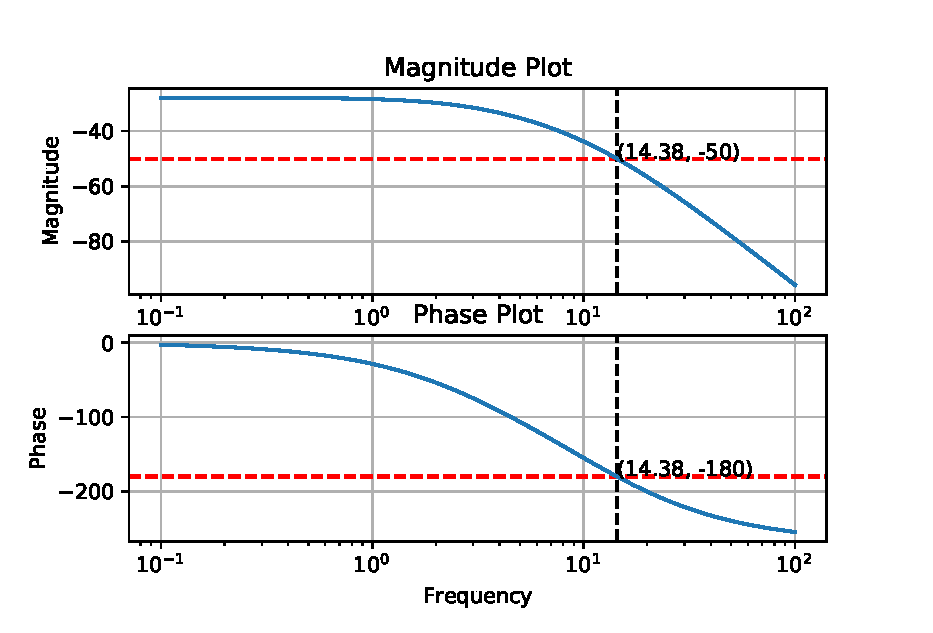
\includegraphics[width=\columnwidth]{./figs/ee18btech11050_1.eps}
\caption{}
\label{fig:ee18btech11050_fig1}
\end{figure}

The following code generates Fig \ref{fig:ee18btech11050_fig1}
\begin{lstlisting}
codes/ee18btech11050_1.py
\end{lstlisting}

\end{enumerate}
